% !TeX document-id = {89cfaf7b-6b10-47b5-8d4d-2cf182e45ca4}
%!TeX TXS-program:compile = txs:///xelatex/[--shell-escape]
\documentclass[11pt,a4paper,oneside,korean]{article}

\usepackage{xetexko}
\usepackage[utf8]{inputenc}
\usepackage[english]{babel}
\usepackage{olymp}
\usepackage{graphicx}
\usepackage{amsmath}
\usepackage{amssymb} 
\usepackage{textcomp}
\usepackage{framed}
\usepackage{color} % for colored text
\usepackage{import} % for changing current dir
\usepackage{epigraph}
\usepackage{daytime} % for displaying version number and date
\usepackage{wrapfig} % for having text alongside pictures
\usepackage{verbatim}
\usepackage{array} % compatibility check
\usepackage{multirow}
\usepackage{pdfpages}
\usepackage{enumitem} % for item environment line spacing
\usepackage{skh2019}
%\usepackage{hangulfontset}

\graphicspath{{./images/}}
\renewcommand{\baselinestretch}{1.4}
\contest
{2019 숭고한 연합 Algorithm Camp Contest - 중급반}%
{숭실대학교}%
{2019.08.09}%

\newcommand*{\NoInputFileName}{}
\newcommand*{\NoOutputFileName}{}

\binoppenalty=10000
\relpenalty=10000
\exhyphenpenalty=10000

%\setmainfont{Noto Sans}
%\setmainhangulfont{Noto Sans CJK KR}
%\setmonofont{D2Coding}

\begin{document}
    %\raggedbottom
    %\displayauthorinfootertrue
    %\intentionallyblankpagestrue
    
    \begin{titlepage}
        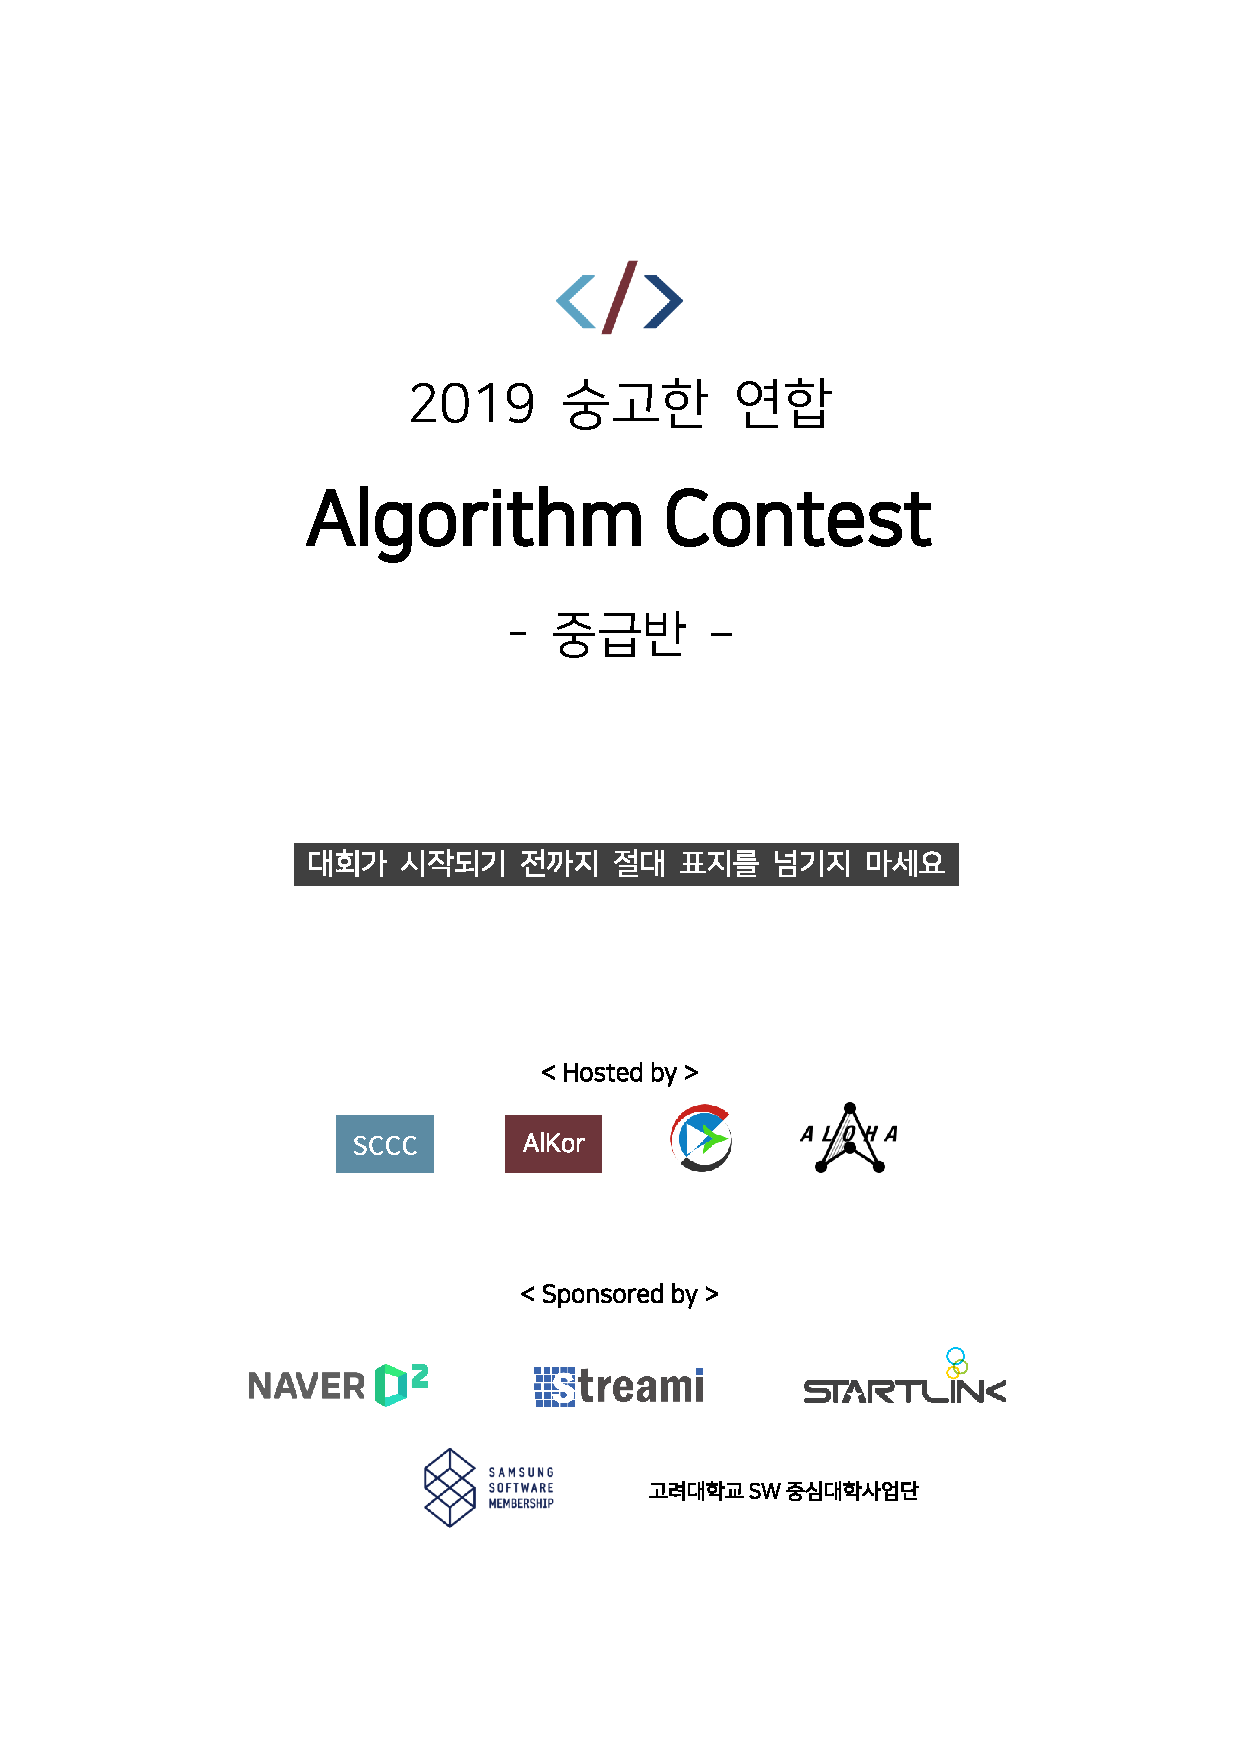
\includepdf[pages=-, pagecommand={\thispagestyle{empty}}, offset=75 -75]{./cover/skh_2019_cover_div2.pdf}
    \end{titlepage}
    \begin{figure}[h]
        \centering
        
\includegraphics[height=0.12\textheight]{./logo-cropped.png}
    \end{figure}
    \skhintro
    {
    
    \begin{table}[h]
    \sffamily\Large
    \renewcommand{\arraystretch}{1.2}
        \begin{tabular}{cl}
        A & 이건 꼭 풀어야 해! \\
        B & 무한부스터 \\
        C & 이진수 변환 \\
        D & 백도어 \\
        E & FLEX \\
        F & 통신망 분할 \\
        G & 트리의 외심 \\
        \end{tabular}
    \end{table}
    }

    \skhintroctd
    
    \newpage
    
    \import{"./problems/"}{begin-ps-must.tex}           % 이건 꼭 풀어야 해!
    \import{"./problems/"}{begin-dp-booster.tex}        % 무한부스터
    \import{"./problems/"}{free-inter-binary.tex}       % 이진수 변환
    \import{"./problems/"}{inter-dist-backdoor.tex}     % 백도어
    \import{"./problems/"}{inter-dp-flex.tex}           % FLEX
    \import{"./problems/"}{inter-disjoint-network.tex}  % 통신망 분할
    \import{"./problems/"}{inter-lca-center.tex}        % 트리의 외심
\end{document}
